\documentclass[12pt]{article}
\usepackage[T1]{fontenc}
\usepackage[polish]{babel}
\usepackage[utf8]{inputenc}
\usepackage{lmodern}
\usepackage{float}
\selectlanguage{polish}
\usepackage{graphicx}
\usepackage{hyperref}
\title{I ty możesz zostać magistrem}
\date{\today}


\begin{document}	
\maketitle
\tableofcontents

\section{Baza Bernsteina}
Baza Bernsteina ze względu na świetne właściwości numeryczne i geometryczne jest szeroko stosowana w systemach CAD/CAM pomimo faktu, że nie jest trójkątna (traingular ???) i nie jest najszybsza w obliczeniach.\\

Ważne właściwości Bazy Bernsteina:
\begin{itemize}
	\item Formują bazę w $n+1$ wymiarowej przestrzeni $w^{n}$ wszystkich wielomianów stopnia nie większego niż $n$.
	\item Sumują się do 1 dla każdego $t \in R$
	\item Są nieujemne w przedziale $[0,1]$ i dodatnie w $(0,1)$.
	\item Sa symetryczne, tzn. $B^{n}_{i=0...n}(t) = B^{n}_{n-1}(1-t)$
\end{itemize}

\subsection{Algorytm de Casteljau}
Algorytm de Casteljau służy do obliczania wartości wielomianów w Bazie Bernsteina. Jest stabilny numerycznie. 
Niewielkim kosztem możemy uzyskąć nie tylko wartość, ale i pochodną w punkcie. Należy odczytać obie wartości algorytmu dla $n-1$ odjąć je i pomnożyć przez $n$.

\subsection{Twierdzenie Weierstrassa}
Każdą funkcję ciągłą o wartościach rzeczywistych na przedziale domkniętym $[a,b]$ można przybliżyć jednostajnie z dowolną dokładnością wielomianami Bernsteina. Im więcej punktów kontrolnych, tym większa dokładność.

\subsection{Baza Hermite'a}
Jeżeli znamy wartości na krańcach przedziału i znamy wartości pochodnych w tych punktach, to podstawiamy do wzoru i mamy aproksymację funkcji na przedziale.
\subsection{Baza Lagrange'a}
Baza nie jest triangularna (???). Można w niej interpolować.
Wielomiany Lagrange'a pozwalają nam na interpolacje punktów, bez potrzeby rozwiązywania układów współrzędnych.
\subsection{Węzły Czebyszewa}
Interpolacja w węzłach Czebyszewa jest prawie najlepsza (znika efekt Rungego).

\section{Piecewise polynomials}
\subsection{Baza B-Spline}
They are much more complex. There are two interesting properties that are not part of the Bézier basis functions, namely: (1) the domain is subdivided by knots, and (2) basis functions are not non-zero on the entire interval. In fact, each B-spline basis function is non-zero on a few adjacent subintervals and, as a result, B-spline basis functions are quite "local".

\setcounter{section}{22}
\section{Metody interpolacji obrotów}
\begin{enumerate}
	\item LERP
	\item SLERP
	\item Liniowa interpolacja kątów Eulera
	\item SQUAD - interpolacja sekwencji orientacji za pomocą wzoru
\end{enumerate}

\section{Aproksymacja obszaru obrobionego}
Obszar obrobiony możemy aproksymować za pomocą paraboloidy ściśle stycznej. 
$$d(\Delta x, \Delta y) = \frac{1}{2} [\Delta x, \Delta y] \textbf{D}  [\Delta x, \Delta y]^{T}$$
gdzie D to dwuforma (przekształcenie dwuliniowe) określająca przybliżaną powierzchnię.\\
Typowe zadanie z PUSNu: jest dana powierzchnia w postaci implicite. Sprawdź jaki maksymalny promień freza nie spowoduje podcięć lub o ile musimy się przesuwać, żeby frezować z zadaną tolerancją (żeby rowki miały maksymalnie jakąś wysokość).\\
Robimy dwuformę powierzchni i freza i je odejmujemy. Sprawdzamy czy ta dwuforma jest dodatnio określona ($X^{T}DX$ > 0, dla każdego $X$). Jeżeli tak, to nie ma podcięć. Jeżeli nie, to podcięcia mogą wystąpić, ale nie muszą (chyba trzeba sprawdzić kierunki, które chcemy frezować ???).
 
 \section{Lokalne i globalne algorytmy programowania 3C}
 Lokalne - tak jak frezowaliśmy nasze modele. APT to język do programowania urządzen sterowanych numerycznie (czyli do robienia ścieżek). Wyróżniamy w nim procedury TO/ON/PAST/TANTO (TANgential TO) oraz drive surface, part surface i check surface. PS - frezujemy stycznie do niej, DS - prowadzimy frez stycznie do niej, CS - na niej się zatrzymujemy.\\
Lokalne metody nie gwarantują ścieżek bez podcięć (collision free tool paths). Natomiast metody globalne wykluczają kolizje z ostatecznym kształtem obrabianej części. Globalne metody projektujemy poprzez wyznaczenie ITO (Inverse Tool Offset). Robimy sumę Minkowskiego przeszkód z odwórconym narzędziem w przestrzeni konfiguracji.
 
 \section{Metody rozwiązywania zadania odwrotnego prostych łańcuchów kinematycznych}
 
\setcounter{section}{34}
\section{Interpolacja i aproksymacja w bazach B-spline}
\hyperlink{Prezentacja}{http://www.cad.zju.edu.cn/home/zhx/GM/009/00-bsia.pdf} 


\section{Powierzchnie obciętę i standard IGES}
Standard IGES jest standardem międzynarodowym dotyczącym danych topologicznych, geometrycznych i niegeometrzyczne (np. materiały, cechy użytkowe). Na podstawie tego standardu powstał również format pliku o tej samej nazwie pozwalający na zapisanie ponad 150 różnych typów obiektów, np. powierzchni trymowanych.

Powierzchnie obcięte składają się z dwóch części: powierzchni bazowej oraz krzywych trymowania, które wyznaczają obszary trymowania.

\section{Struktury danych reprezentacji B-rep}
%Boundary representation of models are composed of two parts: topology and geometry (surfaces, curves and points). The main topological items are: faces, edges and vertices. A face is a bounded portion of a surface; an edge is a bounded piece of a curve and a vertex lies at a point. Other elements are the shell (a set of connected faces), the loop (a circuit of edges bounding a face) and loop-edge links (also known as winged edge links or half-edges) which are used to create the edge circuits. The edges are like the edges of a table, bounding a surface portion. 
Aby uniknąć częstych obliczeń takich jak np, sprawdzenie czy punkt leży na krzywej warto zapamiętywać informacje przy tworzeniu tych struktur.


Boundary representation składa się z dwóch części: topologii oraz geometrii (powierzchnie, krzywe oraz punkty). Główne elementy topologii to: ściany (faces), krawędzie i wierzchołki. Inne elementy to powłoka (shell) - zbiór połączonych ścianek, pętla - cykl krawędzi ograniczającej ściankę, lopp-edge links (znane także jako skrzydlaczki???) - służą do tworzenia cykli z krawędzi (edge circuits). 

\begin{figure}[H]
	\centering
	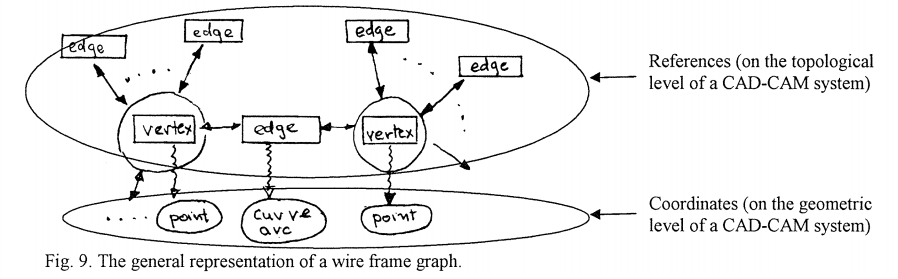
\includegraphics[scale=0.5]{Pictures/brep}
	\caption{B-rep od prof. Marciniaka}
\end{figure}

\subsection{Porównanie CSG}
CSG jest drzewem i zapamiętuje kolejne operacje wykonane na prymitywach. Jest budowane z prymitywów i podstawowych operacji boolowskich.\\
B-rep ma większą liczbę operacji, np. wyciągnięcie (extrusion) i wygładzenie krawędzi (chamfer), co pozwala na bardziej "ludzkie" tworzenie modeli.

\section{Metody lokalizacji obliczeń geometrycznych}
Przykładem problemu lokalizacji obliczeń geometrycznych jest wykrycie kolizji dwóch złożonych obiektów. Zamiast sprawdzać każdy ich element z każdym, chcemy uprościć obliczenia, odrzucając obszary, w których wiemy, że kolizja raczej nie zajdzie.

\subsection{Drzewo BSP}
Drzewo BSP (binary space partitioning) - dzielimy przestrzeń na dwie mniejsze dowolną płaszczyzną.\\
Drzewo kd - dzielimy przestrzeń na dwie mniejsze płaszczyzną ortogonalną do osi układu.\\
Octree - dzielimy przestrzeń 3D na osiem sześcianów.\\

\begin{figure}[h!]
	\centering
	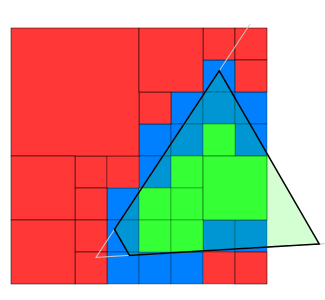
\includegraphics[scale=0.5]{Pictures/octree}
	\caption{Przykład quadtree}
\end{figure}

\section{Struktura systemu do projektowania przez podanie ograniczeń}
Zamiast sekwencyjnie rysować scenę (np. najpierw wstawiamy punkt, potem okrąg, który ma w nim środek, następnie styczną itp.), podajemy układ równań, który definiuje nam całą scenę. Jeżeli zmiennych mamy więcej niż równań to część zmiennych musi wprowadzić użytkownik jako dane wejściowe.


\section{Pojęcie naprężenia w materiale. Wektor i tensor naprężenia}
Naprężenie $\sigma$ (ang. stress) to miara gęstości powierzchniowych sił wewnętrznych, występujących w pewnym punkcie przekroju ośrodka ciągłego (ciała wolumetrycznego). Jednostką naprężenia jest paskal. Reprezentowany jako trójwymiarowy symetryczny tensor drugiego rzędu.

Wektor naprężenia $t$ to gęstość sił działających na element powierzchni w danym punkcie $P \in B$, gdzie $B$ to ośrodek ciągły (ciało). W przypadku sił wewnętrznych wartość $t$ w punkcie $P$ zależy od przekreju. Wektor $t$ jest skierowany wzdłuż wersora normalnego $n$ do powierzchni.

Po prostu: $t$ to wektor z kierunkiem $n$, a $\sigma$ to jego wartość.

\begin{equation}
t_{i} = \sigma_{ij}n_{i}
\end{equation}



\begin{figure}[H]
	\centering
	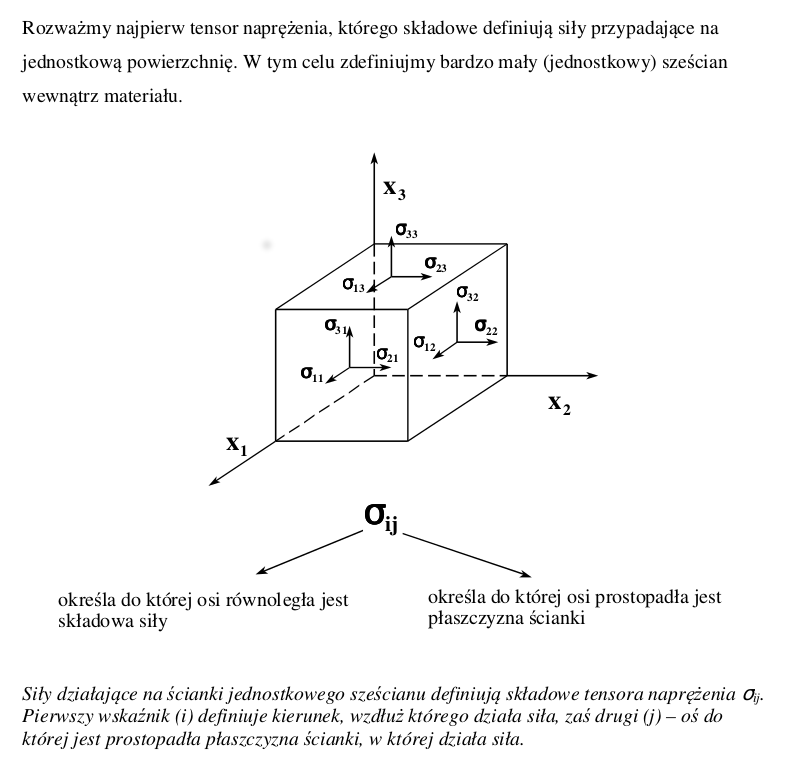
\includegraphics[scale=0.5]{Pictures/stress.png}
	\caption{}
\end{figure}

\section{Algebra Zewnętrzna}

\subsection{Forma różniczkowa (k-forma)}

\subsection{Pochodna zewnętrzna}

\subsection{Dywergencja}
Dywergencja pola wektorowego to operator różniczkowy przyporządkowujący trójwymiarowemu (dwuwymiarowy też) polu wektorowemu pole skalarne będące formalnym iloczynem skalarnym operatora nabla $\nabla$ z polem. 

Dywergencja to miara ilości strumienia wchodzącego lub wychodzącego z punktu. Dywergencja to tempo ekspansji (ang. expansion, positive divergence) lub skurczania (ang. contraction, negative divergence) się strumienia.

Jeśli dany punkt zobaczy strumień, który do niego wchodzi to zacznie krzyczeć, że wszystko się zbliża (ang. negative divergence). Jeśli dany punkt zobaczy strumień, który z niego wychodzi to zacznie krzyczeć, że wszystko sie od niego oddala (ang. positive divergence).

\begin{figure}[H]
	\centering
	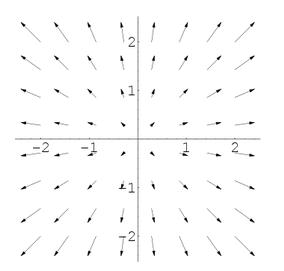
\includegraphics[scale=1.0]{Pictures/vector_field_div.png}
	\caption{Przykład pola wektorowego pokazujący prędkość strumienia cieczy. Strumień oddala się od początku ukladu współrzędnych (ekspansja). Ta ekspansja (ang. expansion) jest udowodniona przez dodatnią wartość dywergencji div F}
\end{figure}

\subsection{Twierdzenie Stokesa}
Całka formy różniczkowej (k-formy) $\omega$ na brzegu $\partial \Omega$ jakieś rozmaitości (manifold) jest równa całce pochodnej zewnętrznej $d \omega$ na całości $\Omega$

\begin{equation}
\int_{\partial \Omega} \omega = \int_{\Omega} d \omega
\end{equation}

Twierdzenie Gaussa-Ostrogradskiego, podstawowe twierdzenie rachunku całkowego (Fundamental theorem of calculus) i twierdzenie Greena są specjalnymi przypadkami twierdzenia Stokesa.

Tw. Stokesa umożliwia nam zamianę całki powierzchniowej na objętościową (i na odwrót)

\subsection{Twierdzenie Gaussa-Ostrogradskiego}

Znane także jako twierdzenie o dywergencji (Divergence theorem).
Specjalny przypadek tw. Stokesa, w którym funkcja podcałkowa po objętości to dywergencja pola wektorowego $F$

\begin{equation}
\int_{V} (\nabla \cdot F) dV = \int_{\partial V} (F \cdot n) dA
\end{equation}

$F$ to pole wektorowe zdefiniowane w sąsiedztwie $V$. $n$ to pole normalnych (skierowanych na zewnątrz, ang. outward) do brzegu $\partial V$.

Załóżmy, że chcemy napompować koło samochodowe, które jest idealną bryła sztywną (koło nie rozszerzy się po dodaniu powietrza). Co się stanie z powietrzem w środku koła? Powietrzne w środku koła skurczy się.

Jeśli $F$ to pole wektorowe reprezentujące strumień cieczy to dywergencja div $F$ reprezentuje ekspansję lub skurczanie sie tej cieczy. Tw. o dywergencji mówi, że całkowita ekspansja strumienia cieczy w jakims trójwymiarowym regionie $V$ jest równa całkowitemu strumieniowi cieczy na zewnątrz brzegu $V$.

W naszym przykładzie koło stanowi region $V$. Pompowanie powietrza do środka koła w kierunki przeciwnym do normalnej $n$ daje nam ujemna wartość $\int_{\partial V} (F \cdot n) dA$. Co oznacza, że wartość $\int_{V} (\nabla \cdot F) dV$ też jest ujemna, co oznacza, że powietrze skurczyło się. Dokładnie to co założyliśmy.

\end{document}